% This is the code that generates the slides we'll use for this section.
% If you'd simply like to view the slides, please open slides.pdf


\documentclass[10pt, aspectratio=169]{beamer}

\makeatletter
  \def\beamer@calltheme#1#2#3{%
    \def\beamer@themelist{#2}
    \@for\beamer@themename:=\beamer@themelist\do
    {\usepackage[{#1}]{\beamer@themelocation/#3\beamer@themename}}}

  \def\usefolder#1{
    \def\beamer@themelocation{#1}
  }
  \def\beamer@themelocation{}

\usefolder{../__resources__/beamer_theme}
\usetheme{nathan}

\addtobeamertemplate{navigation symbols}{}{%
    \usebeamerfont{footline}%
    \usebeamercolor[fg]{footline}%
    \hfill%
    \insertframenumber/\inserttotalframenumber
}

\title{Computational Decision Making for Regular People}
\subtitle{02: Python Crash Course}
\date{October 22, 2024}

\usepackage[font=tiny,labelfont=bf]{caption}
\usepackage{caption}
\captionsetup[figure]{labelformat=empty}

\usepackage{listings}

\begin{document}

\begin{frame}
    \maketitle
\end{frame}

\begin{frame}{Today's Outline}
    \begin{columns}
        \begin{column}{0.5\textwidth}
            \begin{enumerate}
                \item What is Python / Anaconda?
                \item Installing Python (and necessary packages)
                \item Writing your first Python code
                \item Introduction to Jupyter Lab
                \item Key Python concepts
                \begin{enumerate}
                    \item Variables (integers, floats, strings, lists)
                    \item Loops
                    \item Functions
                    \item Data Structures
                \end{enumerate}
                \item Key Python packages
                \begin{enumerate}
                    \item Numpy
                    \item Matplotlib
                    \item Pandas (if there is time)
                \end{enumerate}
            \end{enumerate}
        \end{column}
        \begin{column}{0.5\textwidth}
            \begin{figure}
                
\includegraphics[width=0.95\linewidth]{PythonLogo.png}
            \end{figure}
        \end{column}
    \end{columns}
    \vspace{0.4cm}
    \textit{NOTE: Today's class might feel like a firehose. Don't worry if you don't perfectly grasp everything today. You'll have plenty of time to practice.}
\end{frame}

\begin{frame}[t]{What is Python / Anaconda?}
    \begin{columns}[t]
        \begin{column}[t]{0.5\textwidth}
            What is Python?
            \begin{itemize}
                \item Python is a computer language (a set grammatical rules) in conjunction with a computer program that reads written statements and performs the commands written therein.
                \item You can \underline{write} Python code in any place you can write words (even on paper, if you want).
                \item But you can only \underline{execute} Python code in the Python software package.
            \end{itemize}
        \end{column}
        \begin{column}{0.5\textwidth}
            What is Anaconda (a.k.a. "conda")?
            \begin{itemize}
                \item The Python language normally is used in conjunction with a bunch of pre-built packages that allow you to do a variety of things.
                \item Anaconda is another computer program that helps you manage your installation / version of Python in addition to all the other libraries you may have installed.
                \item One of the easiest ways to download, maintain, and get packages for Python is through Anaconda.
                \item Anaconda comes with a bunch of extra bells and whistles that we con't need for this course. So we'll use a smaller version called "miniconda".
            \end{itemize}
        \end{column}
    \end{columns}
\end{frame}

\begin{frame}{Installing Python (Anaconda)}
    \begin{enumerate}
        \item Visit the following website in your internet browser: https://docs.anaconda.com/miniconda/miniconda-install/
        \item Follow the instructions relevant to your operating system (Windows or Mac)
        \begin{itemize}
            \item Remember (e.g. write down) the key steps to run the anaconda program once it's been installed. You'll need to run this program every time you want to run and/or edit any Python scripts. I'll refer to this program as the "command line".
            \item Windows: Start Menu \textgreater\ Anaconda Prompt
            \item Mac: Terminal Application (e.g. Command + Space \textgreater\ Terminal)
        \end{itemize}
        \item Copy and Paste these commands into the command line to install all the packages we'll need for this course (click "Enter" between commands).
        \begin{itemize}
            \item conda install -c conda-forge jupyterlab
            \item conda install numpy
            \item conda install conda-forge::matplotlib
            \item conda install -c conda-forge pyomo
            \item conda install anaconda::pandas
            \item pip install highspy
            \item pip install ipopt
        \end{itemize}
    \end{enumerate}
\end{frame}

\begin{frame}{Writing Your First Python Code}
    \begin{itemize}
        \item Python commands can be executed in bug batches (called scripts) or one-by-one from the command line.
        \item We'll cover your to write scripts later
        \item For now, in the command line, type "python" followed by Enter.
        \item You'll notice that the command line looks like it's changed. You should now see three '\textgreater\textgreater\textgreater' characters followed by a blinking block. This is the "Python shell" anything you type here will be executed as a Python command.
        \item The easiest Python command to write is as follows. Type this command and click Enter.
        \begin{itemize}
            \item print("Hello World")
        \end{itemize}
        \item You should see "Hello World" repeated back to you. The "print" command tells Python to print whatever you tell it to your screen. In this case, we told Python to print the message "Hello World".
        \item To exit out of the Python shell, type "quit()" followed by Enter.
        \item This should return you to the normal command line.
    \end{itemize}
\end{frame}

\begin{frame}{Introduction to Jupyter Lab}
    \begin{itemize}
        \item Typing commands like this one by one into the Python shell can get really tedious.
        \item Jupyter Lab is a nice program that has a graphical user interface that lets you see your Python code, it's output, and several other useful options all in an organized way.
        \item We installed Jupyter Lab a couple of slides ago using Anaconda.
        \item To launch Jupyter Lab, type "jupyter-lab" followed by Enter.
        \begin{itemize}
            \item It may ask you which internet browser you'd like to use, or it may prompt you to copy and paste a URL into your internet browser. Unless an internet browser tab automatically opens up, follow the instructions that get written to the screen.
        \end{itemize}
        \item Jupyter Lab organizes your python code and it's output into one concise file called a "Notebook". Notebooks are nice since they allow you to combine Python code, written text, images, etc. all in one place.
    \end{itemize}
\end{frame}

\begin{frame}{Opening up Lecture Materials}
    \begin{itemize}
        \item To download all the Jupter Notebooks we'll use for the rest of the course, follow these instructions.
        \item Go to the course website: https://github.com/NathanDavisBarrett/ComputationalDecisionMakingCourse
        \item Click on the green "\textless\textgreater\ Code" Button.
        \item Click on Download ZIP from the dropdown menu that appears.
        \item Open up the file that is downloaded and extract the "ComputationalDecisionMakingCourse" folder to somewhere on your computer that you'd like to store it.
        \item Back in Jupyter Lab, there should be a file navigation bar on the right-hand side of the internet browser tab. Use this file navigation bar to navigate to the ComputationalDecisionMakingCourse folder you just extracted.
        \item Open up the 02\_PythonCrashCourse folder and double-click on the "Lecture\_02\_Notebook.ipynb" file. This should open the Jupyter Notebook we'll use for the rest of today.
    \end{itemize}
\end{frame}

\begin{frame}{Python: Basic Arithmetic}
    $$5 \times 5 = 25$$

    $$12 \times 12 = 144$$

    $$123 \times 7 = ?$$

    $$14 \times 17 = ?$$

    \vspace{1cm}
    \begin{center}
        print(123 * 7)

        print(14 * 17)   
    \end{center}
\end{frame}

\begin{frame}{Python: Variables}
    \begin{itemize}
        \item variableName $=$ value
    \end{itemize}

    \begin{center}
        \begin{tabular}{|c||c|c|}
            \hline
            Type & Description & Syntax \\
            \hline \hline
            int & An integer number & A number with no decimal in it\\
            \hline
            float & A "floating point" (a.k.a. decimal) number & A number with a decimal in it \\
            \hline
            char & An alphabetic character & A single character in single quotes\\
            \hline
            str & A string of alphabetic characters & Several characters in double quotes\\
            \hline
            bool & A boolean True or False (binary 0 or 1) value & "True" or "False\\
            \hline
        \end{tabular}
    \end{center}

    \begin{columns}
        \begin{column}{0.5\textwidth}
            \begin{itemize}
                \item Exercises:
                \begin{enumerate}
                    \item Create a variable named 'x' and assign it a value of 37
                    \item Create a variable named 'y' and assign it a value of 15.2
                    \item Create a variable named 'z' and assign it a value of 'x + y'
                    \item Print the value of 'z'
                \end{enumerate}
            \end{itemize}
        \end{column}
        \begin{column}{0.5\textwidth}
            \begin{enumerate}
                \item Create a variable named 'name1' and assign it a value of "Joe"
                \item Create a variable named 'age1' and assign it a value of 37
                \item Print the value of 'age1 + name1'. Before you execute the command, what do you think will happen?
                \item Execute the command. What happens?
            \end{enumerate}
        \end{column}
    \end{columns}
\end{frame}

\begin{frame}[t]{Python: Iterable Variables}
    \begin{columns}[t]
        \begin{column}[t]{0.5\textwidth}
            Lists:
            \begin{itemize}
                \item A list of other variables / values
                \item listName = [\_\_elements\_\_]
                \item Access individual elements using listName[index]
                \item "index" is the element's position within the list
                \item \textbf{NOTE:} The creators of Python defined it in such a say what the "$1^{st}$" element in a list is located at index 0.
            \end{itemize}
            \vspace{1cm}
            myList = ["element1","element2","element3"]

            print(myList[0])

            print(myList[2])
        \end{column}
        \begin{column}[t]{0.5\textwidth}
            Sets:
            \begin{itemize}
                \item Very similar to a list but with not specific order.
                \item Thus there are no indices.
                \item setName = \{\_\_elements\_\_\}
            \end{itemize}
            Why the distinction?
            \begin{itemize}
                \item Sometimes the order of a collection of data is important
                \begin{itemize}
                    \item Order within a queue
                    \item When data is corresponding between multiple lists
                    \item When we want values neatly sorted
                \end{itemize}
                \item Other times we specifically don't want things ordered
                \begin{itemize}
                    \item e.g. If I simply wanted a collection of the names of each student in class today.
                \end{itemize}
            \end{itemize}
        \end{column}
    \end{columns}
\end{frame}

\begin{frame}{Python: Functions}
    \begin{itemize}
        \item For when we have a section of code that we're going to need to repeat.
        \item \textbf{Pro Tip:} To keep your code clean and relatively free of errors, try to minimize the amount of copying and pasting that you do.
        \item Syntax:
        \begin{center}
            def functionName(parameters):

                Code to Repeat Here...
        \end{center}
        \item Python keeps track of when a function starts and stops using indentation.
    \end{itemize}
    \vspace{0.25cm}
    \begin{columns}
        \begin{column}{0.5\textwidth}
            print((1+2)/3)

            print((15+14)/5)

            print((38+29)/32)
        \end{column}
        \begin{column}{0.5\textwidth}
            def AddThenDivide(a,b,c):

                \hspace{0.25cm} addedNumbers = a + b

                \hspace{0.25cm} finalResult = addedNumbers / c

                \hspace{0.25cm} return finalResult
            \vspace{0.25cm}

            print(AddThenDivide(1,2,3))

            print(AddThenDivide(15,14,5))
            
            print(AddThenDivide(38,29,32))
        \end{column}
    \end{columns}
\end{frame}

\begin{frame}{Python: Loops}
    \begin{columns}
        \begin{column}{0.5\textwidth}
            print(AddThenDivide(1,2,3))

            print(AddThenDivide(15,14,5))
            
            print(AddThenDivide(38,29,32))

            \vspace{0.25cm}

            There is still a good bit of copy and paste.

            This is where we can use a loop. (\textbf{Exersize})

            \hrule

            \vspace{0.5cm}

            aList = [1,2,3,4,5]

            bList = [6,7,8,9,10]

            \vspace{0.25cm}

            aPlusBList = [0,0,0,0,0]

            for i in range(len(aList)):

                \hspace{0.25cm} aPlusBList[i] = aList[i] + bList[i]

            \hrule
            \vspace{0.5cm}
            aPlusBList = [aList[i] + bList[i]  for i in range(len(aList))]


        \end{column}
        \begin{column}{0.5\textwidth}
            \begin{itemize}
                \item Three key players:
                \begin{itemize}
                    \item A list, set, etc. to iterate over
                    \item A temporary variable to hold each element individually at different times
                    \item Some code we want to repeat for each element
                \end{itemize}
                \item Two different syntaxes:
                \begin{enumerate}
                    \item for tempVar in myList:

                    \hspace{0.25cm} Some Code Here

                    \item $[$Some Code Here for tempVar in myList$]$
                \end{enumerate}
                \item Two related, built-in Python functions:
                \begin{itemize}
                    \item $len(myList)$: Gives the number of elements in myList
                    \item $range(num)$: Produces a list of all integers from 0 to "num"
                \end{itemize}
            \end{itemize}
        \end{column}
    \end{columns}
\end{frame}

\begin{frame}[t]{If/Else Conditions}
    \textit{NOTE: The notion of an if/else condition exists in Python, but NOT in mathematical modeling. We'll cover how to re-create the behavior of an if/else condition in mathematical modeling in a couple of weeks.}

    \begin{columns}[t]
        \begin{column}[t]{0.5\textwidth}
            % \vspace{-1cm}

            Often in logic, and in code, we want to do some things only if a certain condition is or is not met. We do this in Python using a collection of $if$, $else$, and $elif$ statements.

            \vspace{0.25cm}
            Syntax:
            \vspace{0.25cm}

            if condition1:

            \hspace{0.25cm} Do some stuff

            elif condition 2:

            \hspace{0.25cm} Do some other stuff

            else:

            \hspace{0.25cm} Do some other other stuff

        \end{column}
        \begin{column}[t]{0.5\textwidth}
            \vspace{0.15cm}

            \begin{tabular}{|c|c|}
                \hline
                greater than & a \textgreater\ b \\
                \hline
                greater than or equal to & a \textgreater= b \\
                \hline
                less than & a \textless\ b \\
                \hline
                less than or equal to & a \textless= b \\
                \hline
                equal to & a == b\\
                \hline
                not equal to & a != b \\
                \hline
            \end{tabular}

            \vspace{0.25cm}
            a = 5

            b = 3

            if a \textless= b:

                \hspace{0.25cm} print("a \textless= b")

            elif a \textgreater\ b:

                \hspace{0.25cm} print("a \textgreater\ b")

        \end{column}
    \end{columns}
\end{frame}

\begin{frame}{List / Function / Loop / If Exercise}
    \begin{center}
        Please try to complete this exercise on your own.

        I'll circle around and help if anyone needs it.
    \end{center}
\end{frame}

\begin{frame}{Python: Custom Data Structures}
    \textit{A quick note on this topic: Unless you want to, you won't need create any custom data structures in this class. So it's not as important to understand exactly how this is done as much as it is important to realize that these exist. We'll be using lots of "custom" data structures that have been created by other people.}
    \vspace{0.5cm}

    \begin{itemize}
        \item Custom data structures are called classes.
        \item A class can have named variables inside of it.
        \item A class can also have functions inside of it.
    \end{itemize}

    \vspace{0.5cm}

    people = [Person("Joe",37),Person("Sally",41),Person("Jacob",17)]

    \vspace{0.25cm}

    print(people[0].age)

    print(people[2].name)

    people[0].printInfo()
\end{frame}

\begin{frame}{Python Packages}
    \begin{itemize}
        \item We can import other people's code into our code!
        \item Syntax:
        \begin{itemize}
            \item import packageName
            \item import packageName as myPersonalAbbreviation
            \item from packageNAme import specificFunctionName
        \end{itemize}
        \item Important packages we'll use in this course:
        \begin{itemize}
            \item numpy
            \item matplotlib
            \item pandas
            \item pyomo
        \end{itemize}
    \end{itemize}
\end{frame}

\begin{frame}{Numpy}
    \begin{itemize}
        \item A package for all things math 
        \item import numpy as np
        \item Complex math functions like $\sqrt{}$ ("np.sqrt"), $\log{}$ ("np.log")
        \item A very simple way to deal with lists (or at least a custom version of lists called "arrays")
        \begin{itemize}
            \item Arrays can be added, multiplied, divided, etc. automatically implementing element-wise addition, multiplication, division, etc.
            \item Arrays can be automatically generated:
            \begin{itemize}
                \item np.linspace
                \item np.arange
            \end{itemize}
            \item Arrays can be "sliced"
        \end{itemize}
        \item See examples in the Jupyter Notebook
    \end{itemize}
\end{frame}

\begin{frame}{Matplotlib}
    \begin{columns}
        \begin{column}{0.5\textwidth}
            \begin{itemize}
                \item A package for all things plotting or graphing
                \item import matplotlib.pyplot as plt
                \item Most important function: plt.plot()
            \end{itemize}
        
            \vspace{0.5cm}
        
            xData = np.linspace(-10,10,100)
        
            yData = xData * xData
        
            \vspace{0.25cm}
        
            plt.plot(xData,yData)
        \end{column}
        \begin{column}{0.5\textwidth}
            \begin{figure}
                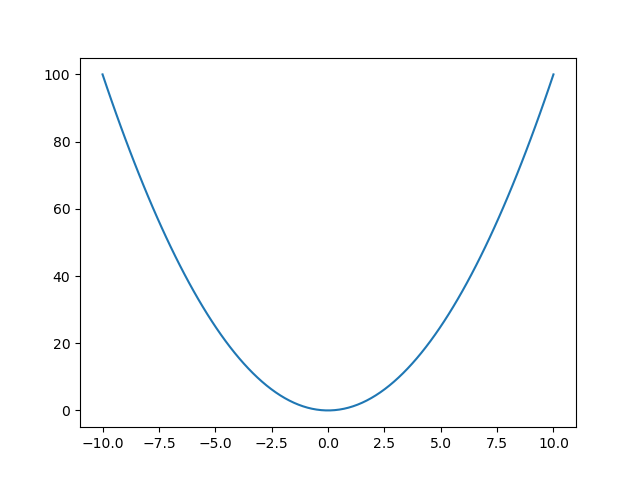
\includegraphics[width=\linewidth]{Quadratic.png}
            \end{figure}
        \end{column}
    \end{columns}

    \vspace{0.25cm}
    \textit{Examples: https://matplotlib.org/stable/api/\_as\_gen/matplotlib.pyplot.plot.html}
\end{frame}

\begin{frame}{Pandas}
    \begin{itemize}
        \item Lots of uses. But in this class we'll mainly use it to import and export excel files.
        \item import pandas as pd
        \item Main Data Structure: pd.DataFrame
        \begin{itemize}
            \item More or less a table. Each column has a specific name.
            \item Columns can be accessed using "myDataFrame[columnName].to\_numpy()"
            \item Write to Excel: "myDataFrame.to\_excel("fileName.xlsx", index=False)
            \item Read from Excel: pd.read\_excel("fileName.xlsx")
        \end{itemize}
        \item See examples in the Jupyter Notebook
    \end{itemize}
\end{frame}

\begin{frame}{Next Class}
    \begin{itemize}
        \item The Pyomo Python Package
        \begin{itemize}
            \item This is the Python package that lets you type in mathematical models (like what we made last class) in almost the same syntax.
            \item Then, using the Pyomo Package, you can have the computer find the optimal solution of those models.
        \end{itemize}
    \end{itemize}

    \vspace{1cm}

    \textit{Again, Today's class might have felt like a firehose. Don't worry if you don't perfectly grasp everything today. You'll have plenty of time to practice as we move forward.}

\end{frame}

\end{document}